\documentclass[svgnames,12pt,aspectratio=149]{beamer}
\mode<presentation>%
{
  \usetheme{Boadilla}
  \setbeamercovered{dynamic}
}
\usepackage[english,french]{babel}
\usepackage[utf8]{inputenc}
\usepackage[T1]{fontenc}
\usepackage{sty/BeamerLille}

\usepackage{graphicx}
\graphicspath{ {./images/} }
\usepackage{tikz}


\usepackage{amssymb,amsfonts}

\author{Gamaliel Moreno}
\title{Redes Neuronales profundas}
\subtitle{Introducción}
\date{Enero-julio 2021}
\institute{\url{gamalielmch@uaz.edu.mx}}


\begin{document}

\begin{frame}[plain]
  \titlepage
\end{frame}
%%%%%%%%%%%%%%%%%%%%%%%%%%%%%%%%%%%%%%%%%%%%%5
\section{Contenido}
\begin{frame}
  \frametitle{Contenido}

  \begin{itemize}
  \item Estructuras  de redes profundas
  \item Capas de combinación 
  \item Capas de activación
  \begin{itemize}
  \item Capas simples
  \item Softmax
  \end{itemize}
  \item Normalización
  \item Funciones de pérdida
  \begin{itemize}
  \item MSE
  \item Entropía cruzada
  \end{itemize}
  \end{itemize}
\end{frame}
%%%%%%%%%%%%%%%%%%%%%%%%%%%%%%%%%%%%%%%%%%%%%5
\section{Estructura de redes profundas}
\begin{frame}
  \frametitle{Estructura genérica de red neuronal profunda}
  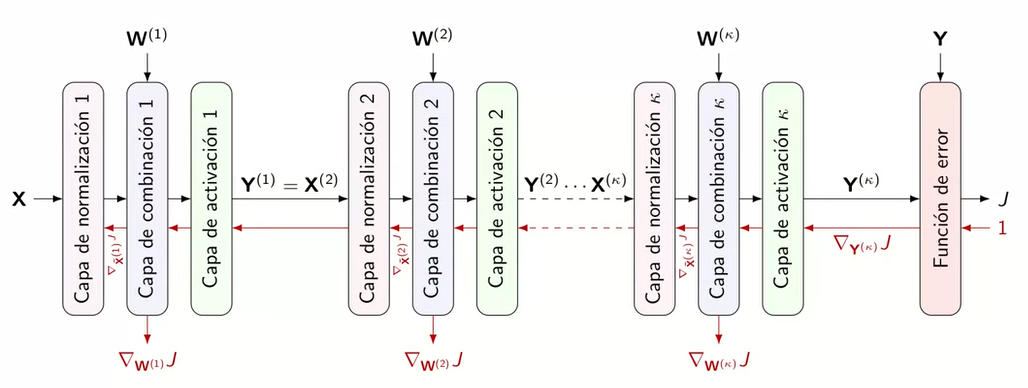
\includegraphics[width=\textwidth]{im1}
\end{frame}
%%%%%%%%%%%%%%%%%%%%%%%%%%%%%%%%%%%%%%%%%%%%%

\begin{frame}
  \frametitle{Contenido}

  \begin{itemize}
  \item Capas de combinación o transferencia
   \begin{itemize}
  \item Capas totalmente conectadas
  \item Capas convolucionales
  \end{itemize}
  \item Capas de activación
  \begin{itemize}
  \item Capas simples
 	\begin{itemize}
  \item Problemas: asimetría postiva, desvanecimiento del gradiente
  \end{itemize}
  \end{itemize}
  \item Normalización
  \item Funciones de pérdida
  \begin{itemize}
  \item MSE
  \item Entropía cruzada
  \end{itemize}
  \end{itemize}
\end{frame}
%%%%%%%%%%%%%%%%%%%%%%%%%%%%%%%%%%%%%%%%%%%%%
\section{Capas de combinación}
\subsection{Capa totalmente conectada}
\begin{frame}
  \frametitle{Capa totalemente conectada o densa}
  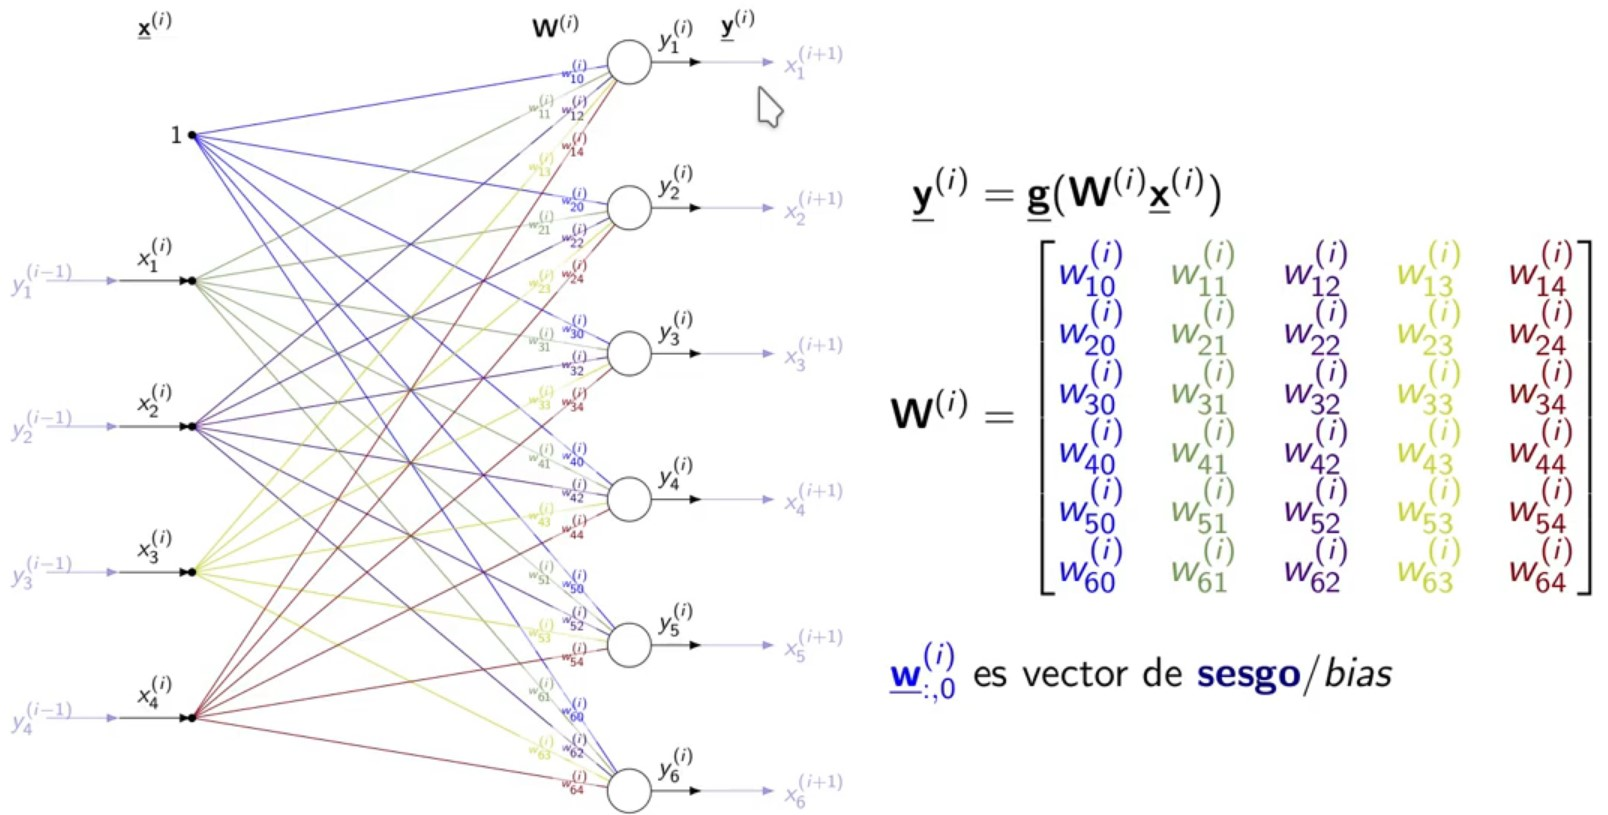
\includegraphics[width= \textwidth]{im2}
  
\end{frame}
%%%%%%%%%%%%%%%%%%%%%%%%%%%%%%%%%%%%%%%%%%%%%
\begin{frame}
  \frametitle{Capa totalemente conectada o densa}
\begin{itemize}
\item Estas capas producen $\boldsymbol{y}$ con una entrada $\boldsymbol{x}$ como combinación lineal:
\begin{equation*}
\boldsymbol{y}=\boldsymbol{W} \begin{bmatrix} 1 \\ \boldsymbol{x} \end{bmatrix}
\end{equation*}
\item Concepto se generaliza para procesar mini-lotes para matriz de diseño $\boldsymbol{X}$ con los datos en sus filas (y salidas en filas de $\boldsymbol{Y} $) 
\begin{equation*}
\boldsymbol{Y}= \begin{bmatrix} \boldsymbol{1} & \boldsymbol{X} \end{bmatrix} \boldsymbol{W}^T
\end{equation*}
\end{itemize}
  
\end{frame}
%%%%%%%%%%%%%%%%%%%%%%%%%%%%%%%%%%%%%%%%%%%%%

\end{document}


%\end{document}

%%% Local Variables:
%%% mode: latex
%%% TeX-master: t
%%% End:
